\documentclass{standalone}
\usepackage{tikz}
\usetikzlibrary{arrows.meta, positioning}

\begin{document}
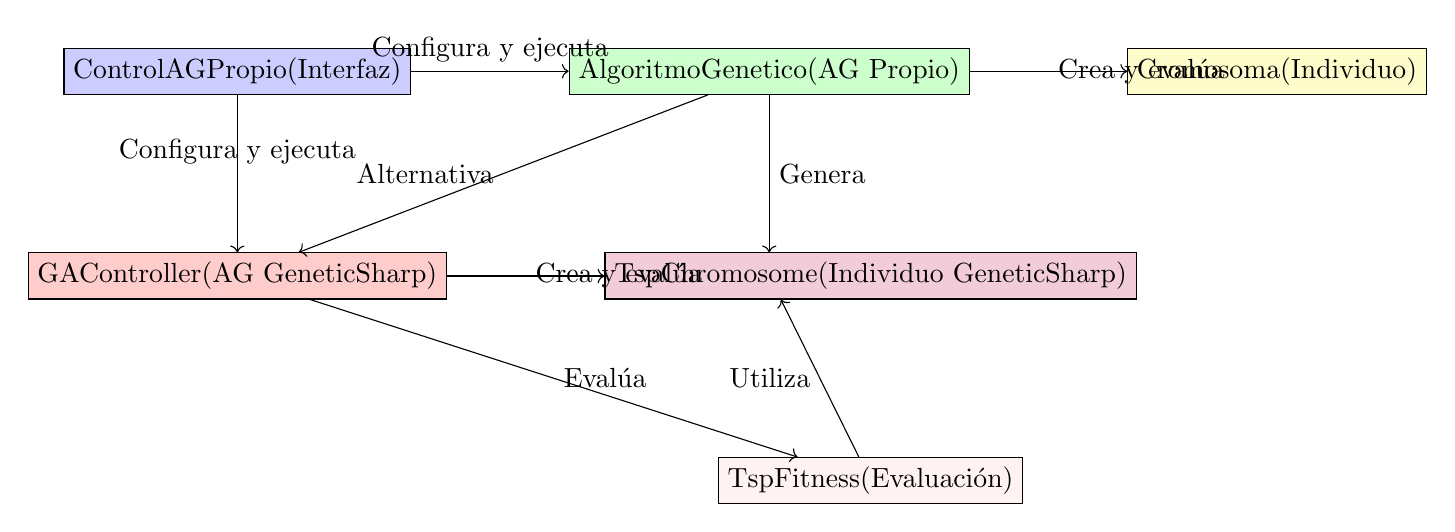
\begin{tikzpicture}[node distance=2cm, auto]
    % Definir nodos para scripts principales
    \node (control) [draw, rectangle, fill=blue!20] {ControlAGPropio\\(Interfaz)};
    \node (algogen) [draw, rectangle, fill=green!20, right=of control] {AlgoritmoGenetico\\(AG Propio)};
    \node (gacontroller) [draw, rectangle, fill=red!20, below=of control] {GAController\\(AG GeneticSharp)};
    \node (cromosoma) [draw, rectangle, fill=yellow!20, right=of algogen] {Cromosoma\\(Individuo)};
    \node (ciudad) [draw, rectangle, fill=orange!20, below=of algogen] {Ciudad\\(Punto TSP)};
    \node (tspchrom) [draw, rectangle, fill=purple!20, right=of gacontroller] {TspChromosome\\(Individuo GeneticSharp)};
    \node (tspfitness) [draw, rectangle, fill=pink!20, below=of tspchrom] {TspFitness\\(Evaluación)};

    % Dibujar conexiones de interacción
    \draw[->] (control) -- (algogen) node[midway, above] {Configura y ejecuta};
    \draw[->] (control) -- (gacontroller) node[midway, above] {Configura y ejecuta};
    \draw[->] (algogen) -- (cromosoma) node[midway, right] {Crea y evalúa};
    \draw[->] (algogen) -- (ciudad) node[midway, right] {Genera};
    \draw[->] (gacontroller) -- (tspchrom) node[midway, right] {Crea y evalúa};
    \draw[->] (gacontroller) -- (tspfitness) node[midway, right] {Evalúa};
    \draw[->] (tspfitness) -- (ciudad) node[midway, left] {Utiliza};
    \draw[->] (algogen) -- (gacontroller) node[midway, left] {Alternativa};
\end{tikzpicture}
\end{document}